To create new project, it is mandatory to create Workflow (WF) template first.
Templates are later accessible for creating similar projects.

To create new template, you need to choose \emph{Projects $>>$
My WF Templates $>>$ Create New WF Template with Wizard} option from the top
menu. The wizard will then
guide you through the process of creating template as explained next in Section
~\ref{section:workflow-template-wizard}.

Another way to create new template is during the creation of New project (
explained later in Section
~\ref{section:create-new-project}) by selecting option
\emph{Blank template} at the list of available templates. Click \emph{Select}
button, and you will be redirected to the \emph {Workflow Template} page, from
where you are entering \emph {Workflow Template Wizard}.

\subsection{Workflow Template Wizard}
\label{section:workflow-template-wizard}
\begin{figure}[hb!]
\centering
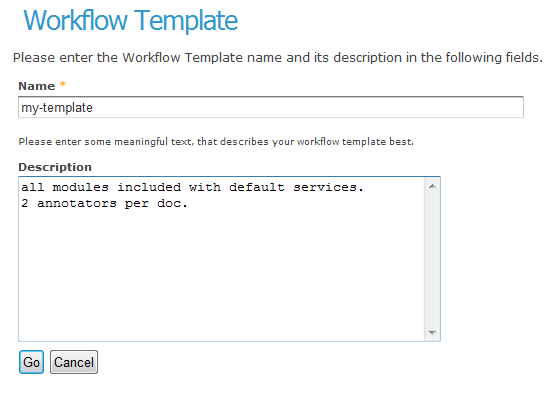
\includegraphics[scale=0.4]{createwftemplate}
\caption{Create New Workflow template}
\label{fig:createwftemplate}
\end{figure}
You need to provide the \emph{name} and \emph{description} of the template.
These two fields will be later used to show overview of the templates and therefore should
contain useful information to help you distinguish between various templates.
Click \emph{Go} button as shown in Figure~\ref{fig:createwftemplate}).

The wizard comprises several steps, the number of which is not fixed as
each of them depends on the preselected options in the previous step.

\begin{figure}[htb]
\centering
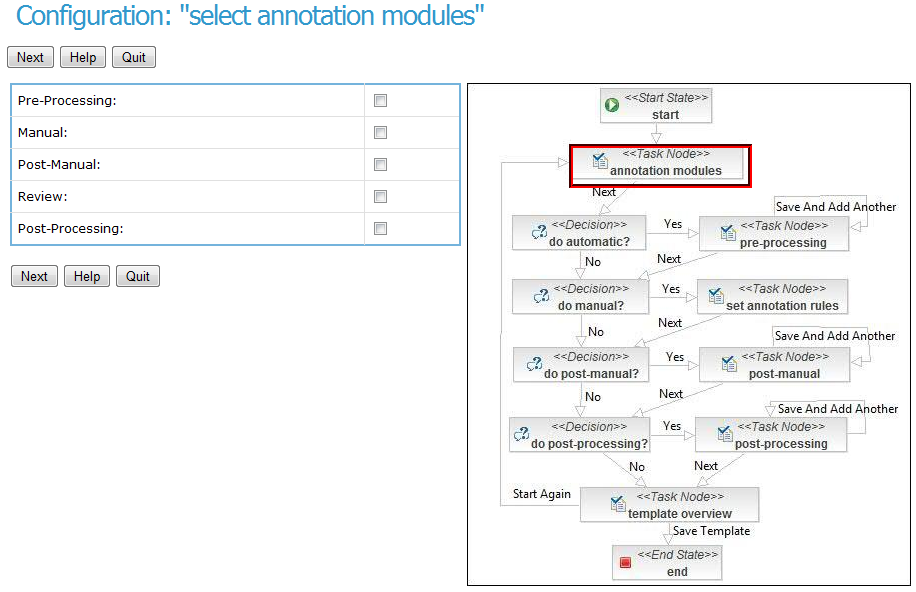
\includegraphics[scale=0.4]{selectannotationmodes}
\caption{Configuration: Select Annotation Modules}
\label{fig:selectannotationmodes}
\end{figure}

During the wizard, the \emph{progress diagram} on the right hand side will
show your progress by highlighting your current step.

The first step is the \emph{Configuration: "select annotation modules"} step,
where you need to choose one or more annotation modules: \emph{automatic},
\emph{manual}, \emph{post-manual}, \emph{review} and/or
\emph{post-processing}, as shown in Figure~\ref{fig:selectannotationmodes}).

Click \emph{Next}. Depending on the chosen modules, the steps to follow
will vary. Here is the detailed explanation of each possible step in case when
all available modules are selected.
\begin{description}
   \item [Pre-processing:] To configure \emph{pre-processing} you need to select
   one or more pre-processing services. When you are done with selection press 
   \emph{Next}. Alternatively you can add as many services as you want to 
   the pipeline by clicking on the button \emph{Save and add another}. This step
  is shown in Figure~\ref{fig:gaspreprocessing}). 
\begin{figure}[hb!]
\centering
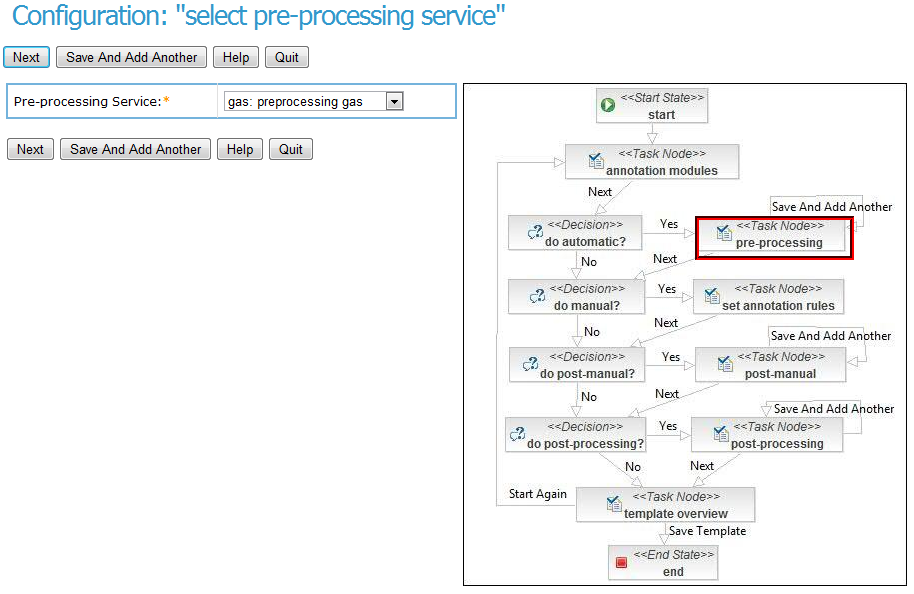
\includegraphics[scale=0.4]{gaspreprocessing}
\caption{Configuration: GAS Pre-processing}
\label{fig:gaspreprocessing}
\end{figure}
    \item  [Manual annotation:] Manual annotation needs a few parameters to be
    specified. This is done in the \emph{Configuration step: "select annotation rules"} 
    as shown inFigure~\ref{fig:selectannotationrules}. Here you will need to:
   \begin{itemize}
       \item select number of annotators per document. For example if you select
       2, each document should be annotated by 2 different annotators;
       \item leave \emph{cancel task allowed} checked; this will allow
       annotators to cancel tasks if they feel unsure about how to annotate the
       document correctly;
       \item leave \emph{anonymous annotation} checked; this will create
       generic annotation set names for annotators (e.g., \emph{annotator1},
       annotator2, etc.) instead of using their usernames. This option is
       useful when you later search annotation sets within documents in
       generalised fashion (for example, using regular expression 'annotator*');
       \item select some of the existing annotation schemas which will be
       loaded inside the Annotation Editor during the process of manual
       annotation (you also have the option to add new schema, if you want).
       \item choose the service which will prepare manual annotation task 
       (copy preprocessed annotations into annotator's annotation set)
   \end{itemize}
 \item  [Post-Manual: and Post-Processing] In \emph{Configuration steps:
   "select post-manual service"}, you can select one or more
   post-manual/post-processing services as shown in
   Figure~\ref{fig:selectpostmanual}. These steps are identical to
   \emph{pre-processing}. The main point is that you can chain services in the order you like 
   and make them executed in a pipeline.
\begin{figure}
\centering
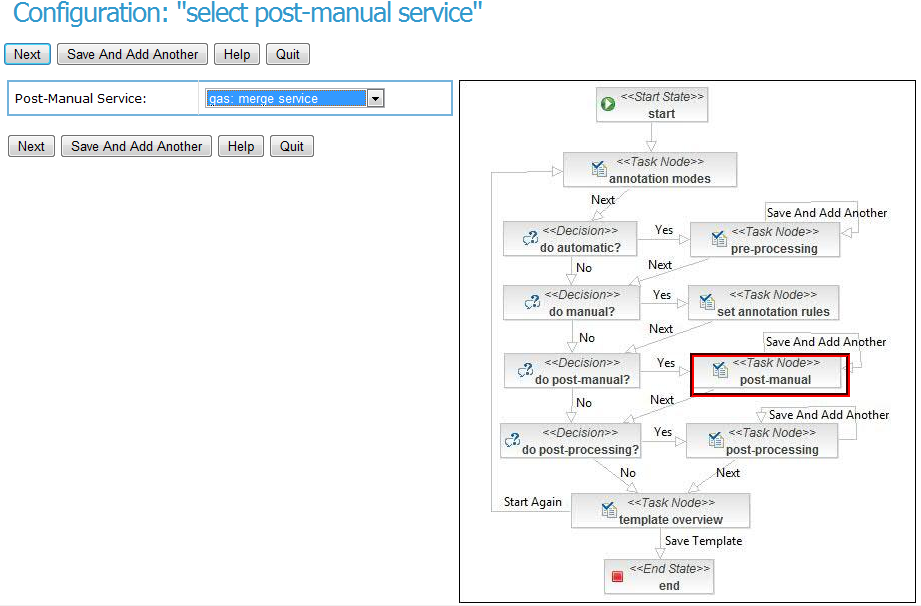
\includegraphics[scale=0.38]{selectpostmanual}
\caption{Configuration: Select Post-Manual}
\label{fig:selectpostmanual}
\end{figure}
\end{description}


From the \emph{Configuration: "template overview"} page
(Figure~\ref{fig:templateoverview}) the template can be saved by clicking on the
\emph{Save template} button. You will be redirected to the
 \emph{My WF Templates} page. Note that if you are not happy with the settings,
 you can repeat the setup procedure by pressing \emph{Start Again} button.
\begin{figure}
\centering
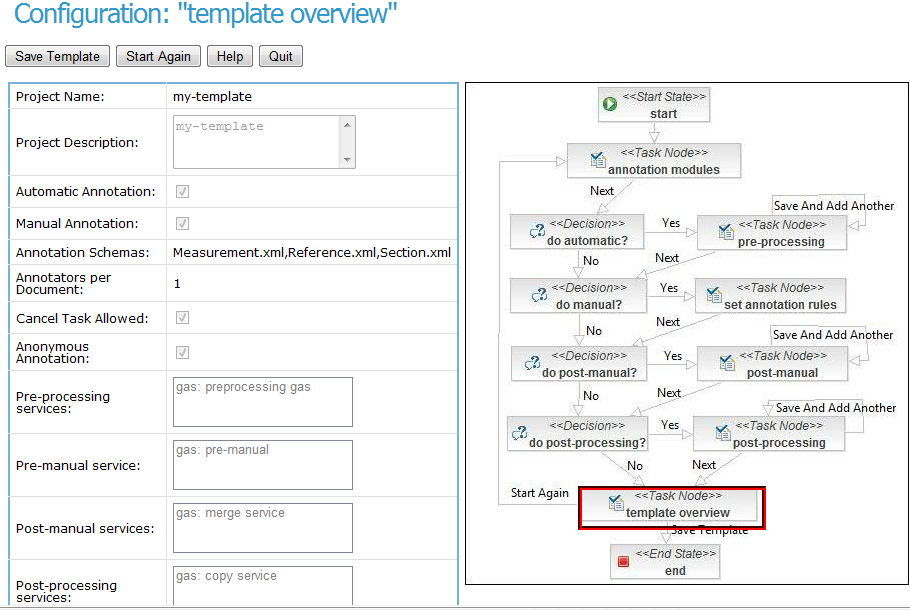
\includegraphics[scale=0.38]{templateoverview}
\caption{Configuration: Template Overview page}
\label{fig:templateoverview}
\end{figure}

At any time you can get more information on the current step or instructions
on how to proceed by hovering over the
 \emph{Help} button. This is especially useful in cases when you are not
sure on how to complete the step.
Quitting the wizard is always possible by pressing the \emph{Quit}
 button. After the warning, and choosing the option \emph{Yes}, the wizard will
 exit, but it can be resumed any time by selecting \emph{Projects $>>$ My WF
 Templates}, and then by clicking \emph{Resume} button for the selected
 template.

